%% BioMed_Central_Tex_Template_v1.06
%%                                      %
%  bmc_article.tex            ver: 1.06 %
%                                       %

%%IMPORTANT: do not delete the first line of this template
%%It must be present to enable the BMC Submission system to
%%recognise this template!!

%%%%%%%%%%%%%%%%%%%%%%%%%%%%%%%%%%%%%%%%%
%%                                     %%
%%  LaTeX template for BioMed Central  %%
%%     journal article submissions     %%
%%                                     %%
%%          <8 June 2012>              %%
%%                                     %%
%%                                     %%
%%%%%%%%%%%%%%%%%%%%%%%%%%%%%%%%%%%%%%%%%


%%%%%%%%%%%%%%%%%%%%%%%%%%%%%%%%%%%%%%%%%%%%%%%%%%%%%%%%%%%%%%%%%%%%%
%%                                                                 %%
%% For instructions on how to fill out this Tex template           %%
%% document please refer to Readme.html and the instructions for   %%
%% authors page on the biomed central website                      %%
%% http://www.biomedcentral.com/info/authors/                      %%
%%                                                                 %%
%% Please do not use \input{...} to include other tex files.       %%
%% Submit your LaTeX manuscript as one .tex document.              %%
%%                                                                 %%
%% All additional figures and files should be attached             %%
%% separately and not embedded in the \TeX\ document itself.       %%
%%                                                                 %%
%% BioMed Central currently use the MikTex distribution of         %%
%% TeX for Windows) of TeX and LaTeX.  This is available from      %%
%% http://www.miktex.org                                           %%
%%                                                                 %%
%%%%%%%%%%%%%%%%%%%%%%%%%%%%%%%%%%%%%%%%%%%%%%%%%%%%%%%%%%%%%%%%%%%%%

%%% additional documentclass options:
%  [doublespacing]
%  [linenumbers]   - put the line numbers on margins

%%% loading packages, author definitions

\documentclass[twocolumn]{bmcart}% uncomment this for twocolumn layout and comment line below
%\documentclass[linenumbers,doublespacing]{bmcart}

%%% Load packages
\usepackage{amsthm,amsmath}
\RequirePackage{natbib}
%\RequirePackage[authoryear]{natbib}% uncomment this for author-year bibliography
%\RequirePackage{hyperref}
\usepackage[utf8]{inputenc} %unicode support
%\usepackage[applemac]{inputenc} %applemac support if unicode package fails
%\usepackage[latin1]{inputenc} %UNIX support if unicode package fails
\usepackage[flushleft]{threeparttable}
\usepackage{upgreek}
\usepackage{amssymb}
\usepackage{url}

%%%%%%%%%%%%%%%%%%%%%%%%%%%%%%%%%%%%%%%%%%%%%%%%%
%%                                             %%
%%  If you wish to display your graphics for   %%
%%  your own use using includegraphic or       %%
%%  includegraphics, then comment out the      %%
%%  following two lines of code.               %%
%%  NB: These line *must* be included when     %%
%%  submitting to BMC.                         %%
%%  All figure files must be submitted as      %%
%%  separate graphics through the BMC          %%
%%  submission process, not included in the    %%
%%  submitted article.                         %%
%%                                             %%
%%%%%%%%%%%%%%%%%%%%%%%%%%%%%%%%%%%%%%%%%%%%%%%%%


% remove this comment before submission
\usepackage{graphicx}
%\def\includegraphic{}
%\def\includegraphics{}



%%% Put your definitions there:
\startlocaldefs
\newcommand{\wolf}[1]{{\textcolor{red}{[Wolf: {#1}]}}}
\newcommand{\elad}[1]{{\textcolor{magenta}{[Elad: {#1}]}}}
\newcommand{\Sint}{\mathbf{S_{int}}}
\endlocaldefs


%%% Begin ...
\begin{document}

%%% Start of article front matter
\begin{frontmatter}

\begin{fmbox}
\dochead{Research}

%%%%%%%%%%%%%%%%%%%%%%%%%%%%%%%%%%%%%%%%%%%%%%
%%                                          %%
%% Enter the title of your article here     %%
%%                                          %%
%%%%%%%%%%%%%%%%%%%%%%%%%%%%%%%%%%%%%%%%%%%%%%

\title{Removing both Internal and Unrealistic Energy-Generating Cycles in Flux Balance Analysis}

%%%%%%%%%%%%%%%%%%%%%%%%%%%%%%%%%%%%%%%%%%%%%%
%%                                          %%
%% Enter the authors here                   %%
%%                                          %%
%% Specify information, if available,       %%
%% in the form:                             %%
%%   <key>={<id1>,<id2>}                    %%
%%   <key>=                                 %%
%% Comment or delete the keys which are     %%
%% not used. Repeat \author command as much %%
%% as required.                             %%
%%                                          %%
%%%%%%%%%%%%%%%%%%%%%%%%%%%%%%%%%%%%%%%%%%%%%%

\author[
   addressref={aff1},                   % id's of addresses, e.g. {aff1,aff2}
   corref={aff1},                       % id of corresponding address, if any
   %noteref={n1},                        % id's of article notes, if any
   email={noor@imsb.biol.ethz.ch}       % email address
]{\inits{EN}\fnm{Elad} \snm{Noor}}


%%%%%%%%%%%%%%%%%%%%%%%%%%%%%%%%%%%%%%%%%%%%%%
%%                                          %%
%% Enter the authors' addresses here        %%
%%                                          %%
%% Repeat \address commands as much as      %%
%% required.                                %%
%%                                          %%
%%%%%%%%%%%%%%%%%%%%%%%%%%%%%%%%%%%%%%%%%%%%%%
\address[id=aff1]{%                           % unique id
  \orgname{Institute of Molecular Systems Biology, Eidgenössische Technische Hochschule}, % university, etc
  %\street{},                                %
  \postcode{8093}                            % post or zip code
  \city{Zürich},                             % city
  \cny{Switzerland}                          % country
}


%%%%%%%%%%%%%%%%%%%%%%%%%%%%%%%%%%%%%%%%%%%%%%
%%                                          %%
%% Enter short notes here                   %%
%%                                          %%
%% Short notes will be after addresses      %%
%% on first page.                           %%
%%                                          %%
%%%%%%%%%%%%%%%%%%%%%%%%%%%%%%%%%%%%%%%%%%%%%%

\begin{artnotes}
%\note{Sample of title note}     % note to the article
\note[id=n1]{Equal contributor} % note, connected to author
\end{artnotes}

\end{fmbox}% comment this for two column layout

%%%%%%%%%%%%%%%%%%%%%%%%%%%%%%%%%%%%%%%%%%%%%%
%%                                          %%
%% The Abstract begins here                 %%
%%                                          %%
%% Please refer to the Instructions for     %%
%% authors on http://www.biomedcentral.com  %%
%% and include the section headings         %%
%% accordingly for your article type.       %%
%%                                          %%
%%%%%%%%%%%%%%%%%%%%%%%%%%%%%%%%%%%%%%%%%%%%%%

\begin{abstractbox}

\begin{abstract} % abstract
Constraint-based stoichiometric models are ubiquitous in metabolic research, with Flux Balance Analysis (FBA) being the most widely used method to describe metabolic phenotypes of cells growing in steady-state. Of the many variants of constrain-based modelling methods published throughout the years, only few have focused on thermodynamic issues, in particular the elimination of non-physical and non-physiological cyclic fluxes. In this work, we revisit two of these methods, namely thermodynamic FBA and loopless FBA, and analyze the strengths and weaknesses of each one. Finally, we suggest a compromise denoted \textit{semi-thermodynamic FBA} (st-FBA) which imposes stronger thermodynamic constrains on the flux polytope compared to loopless FBA, without requiring a large set of thermodynamic parameters as in the case of thermodynamic FBA. We show that st-FBA is a useful and simple way to eliminate thermodynamically infeasible cycles that generate ATP.
\end{abstract}

%%%%%%%%%%%%%%%%%%%%%%%%%%%%%%%%%%%%%%%%%%%%%%
%%                                          %%
%% The keywords begin here                  %%
%%                                          %%
%% Put each keyword in separate \kwd{}.     %%
%%                                          %%
%%%%%%%%%%%%%%%%%%%%%%%%%%%%%%%%%%%%%%%%%%%%%%

\begin{keyword}
\kwd{thermodynamics}
\kwd{flux-balance analysis}
\kwd{loopless}
\kwd{energy-generating cycles}
\end{keyword}

% MSC classifications codes, if any
%\begin{keyword}[class=AMS]
%\kwd[Primary ]{}
%\kwd{}
%\kwd[; secondary ]{}
%\end{keyword}

\end{abstractbox}
%
%\end{fmbox}% uncomment this for twcolumn layout

\end{frontmatter}

%%%%%%%%%%%%%%%%%%%%%%%%%%%%%%%%%%%%%%%%%%%%%%
%%                                          %%
%% The Main Body begins here                %%
%%                                          %%
%% Please refer to the instructions for     %%
%% authors on:                              %%
%% http://www.biomedcentral.com/info/authors%%
%% and include the section headings         %%
%% accordingly for your article type.       %%
%%                                          %%
%% See the Results and Discussion section   %%
%% for details on how to create sub-sections%%
%%                                          %%
%% use \cite{...} to cite references        %%
%%  \cite{koon} and                         %%
%%  \cite{oreg,khar,zvai,xjon,schn,pond}    %%
%%  \nocite{smith,marg,hunn,advi,koha,mouse}%%
%%                                          %%
%%%%%%%%%%%%%%%%%%%%%%%%%%%%%%%%%%%%%%%%%%%%%%

%%%%%%%%%%%%%%%%%%%%%%%%% start of article main body
% <put your article body there>

%%%%%%%%%%%%%%%%
%% Background %%
%%
\section*{Content}
Text and results for this section, as per the individual journal's instructions for authors. %\cite{koon,oreg,khar,zvai,xjon,schn,pond,smith,marg,hunn,advi,koha,mouse}

\section*{Introduction}
The repertoire of genome-scale metabolic reconstructions is growing quickly, with more and more organisms being modelled every year \cite{King2016-it}. Likewise, the list of constraint-based modelling methods is getting longer with more than 100 papers published since 1961 in a rapidly increasing rate \cite{Lewis2012-mu} (see \url{http://cobramethods.wikidot.com/methods}). Flux Balance Analysis (FBA), is arguably the most well-known method to describe possible steady-state fluxes in a growing cell, and typically used to predict biomass yield and reaction essentiality. 

Throughout the years, many extensions have been suggested in order to incorporate different aspects of thermodynamics into constrain-based frameworks \cite{Beard2002-xt, Warren2007-wm, Henry2007-xp, Schellenberger2011-bq, Price2006-ua, Bordel2010-pl, Fleming2010-py, Holzhutter2004-qj, Fleming2009-um, Kummel2006-qn, Henry2006-nt, Hoppe2007-sw, De_Martino2012-cj, Tepper2013-gd, Nolan2006-eg, Nagrath2007-bn, Boghigian2010-vz}.
Two of these methods, \textit{thermodynamic FBA} \cite{Henry2007-xp} and \textit{loopless FBA} \cite{Schellenberger2011-bq} (also known as TMFA and ll-COBRA), define a new list of variables that represent the Gibbs free energy of formation of each metabolite in the system, and add constraints on reaction directionality that correspond to these free energies. Thermodynamic FBA imposes an extra set of constraints defining a range of possible values for each formation energy, and therefore requires many more parameters (which are often difficult to obtain). On the other hand, loopless FBA requires no extra parameters but does not necessarily eliminate all thermodynamically infeasible reactions or pathways. In this paper, we suggest a compromise denoted \textit{semi-thermodynamic FBA} (st-FBA) which imposes stronger thermodynamic constrains on the flux polytope compared to loopless FBA, without requiring a large set of thermodynamic parameters. Finally, we show that st-FBA is a useful and simple way to prevent flux in Energy Generating Cycles (EGCs) -- i.e. thermodynamically infeasible cycles that generate ATP or other energy currencies.

Typically, FBA requires a reconstruction of the metabolic network with $n$ metabolites and $r$ reactions, which is described by a stoichiometric matrix $\mathbf{S} \in \mathbb{R}^{n \times r}$. Some of the reactions in $\mathbf{S}$ are denoted \emph{primary exchange} reactions. These reactions represent the exchange of material between the model and the environment, i.e. input of nutrients and export of by-products. These reactions are not real chemical transformations nor transport reaction, but rather ``conceptual'' constructs that enable the system to be in a non-trivial steady state. Typically, primary exchange reactions have only one product and not substrates, or vice versa (see magenta reactions in Figure \ref{fig:cycles}). Another subset of reactions correspond to \emph{currency exchange} fluxes. These reactions represent the exchange of currency metabolites between different sub-networks (or compartments) in the cell. In the context of this work, we consider only the exchange of energy (e.g. ATP hydrolysis) as currency exchange. For instance, this exchange can be used to model the exchange of energy between the mitochondria (where ATP is generated) and the nucleus (where ATP is used). In bacterial models, where compartments play a minor role, many ATP utilizing processes are lumped into one cytoplasmic reaction called \emph{ATP maintenance} (see green reaction in Figure \ref{fig:cycles}). Finally, all other reactions are considered \emph{internal} reactions, and the sub-matrix of $\mathbf{S}$ corresponding to them is denoted $\Sint$.

\subsection*{Steady-state assumption}
$\mathbf{S}$ relates between the flux vector $v \in \mathbb{R}^{r}$ and the change in metabolite concentrations $x \in \mathbb{R}^{n}$:
\begin{equation}
\frac{dx}{dt} = \mathbf{S} \cdot v\,\,.
\end{equation}
The steady-state assumption imposes a constraint that all concentrations are constant over time, therefore
\begin{equation}\label{eq:st1}
\mathbf{S} \cdot v = 0 \,\,. 
\end{equation}
Most constrain-based applications come with additional constraints on individual fluxes, i.e.
\begin{equation}\label{eq:st2}
\forall i~~~\alpha_i \leq v_i \leq \beta_i\,\,.
\end{equation}


\subsection*{Extreme pathways}
Extreme pathways are convex basis vectors that define the polytope of solutions to the steady-state problem (Equations \ref{eq:st1}-\ref{eq:st2}). In \cite{Schilling2000-rn, Beard2002-xt}, three basic categories of extreme pathways were defined:
\begin{description}
\item[Type I] -- \textit{Primary systemic pathways}, i.e. pathways where at least one primary exchange flux is active.
\item[Type II] -- \textit{Futile cycles}, i.e. pathways where none of the primary exchange fluxes are active, but at least one currency exchange flux is active.
\item[Type III] -- \textit{Internal cycles}, i.e. pathways where none of the exchange fluxes (primary and currency) are active.
\end{description}

\begin{figure}[h!]
	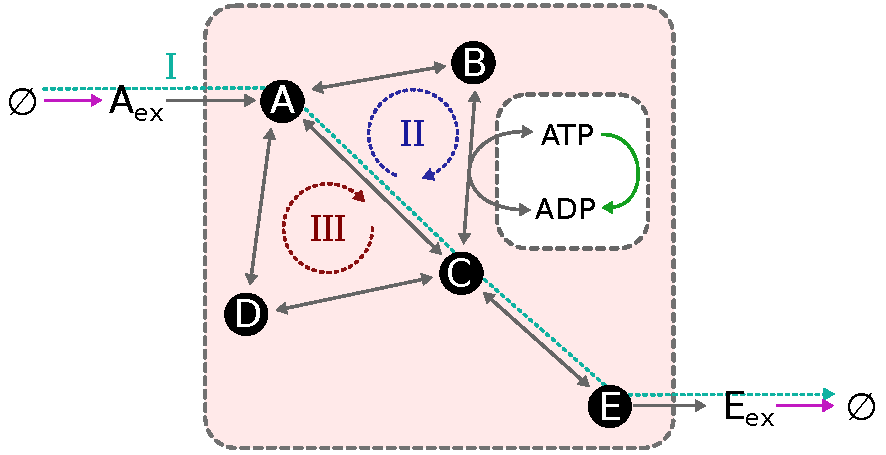
\includegraphics[width=3.1in]{figure1.pdf}
	\caption{\csentence{The Three Types of Extreme Pathways.}
		A small toy model with 8 internal reaction (grey), 2 primary exchange reactions (magenta), and one currency exchange reaction (green). In this simple network, one can identify all three types of extreme pathways. The Type I pathway (connecting between $A_{ex}$ and $E_{ex}$, cyan) is typically the type of solution that most constrain-based models are seeking. The Type II pathway ($A \rightarrow B \rightarrow C \rightarrow A$, blue) is a typical futile cycle, since it does not involve any primary exchange reactions, but does \emph{waste} ATP. The Type III pathway ($A \rightarrow C \rightarrow D \rightarrow A$, red) is called internal since none of its reactions are exchange reactions. An internal cycle will never be thermodynamically feasible.}
    \label{fig:cycles}
\end{figure}
Figure \ref{fig:cycles} demonstrates this classification in a toy model. It is important to note, that this classification depends on the definition of primary and currency exchange reactions, and therefore is not a property of the stoichiometric matrix itself.

In 2011, an extension of FBA was proposed that can eliminate all internal cycles (sometimes called "infeasible loops") from the solution space \cite{Schellenberger2011-bq}. This method is usually referred to as ``loopless'' FBA (ll-FBA). Later, we proved mathematically that this method is both sound and complete \cite{Noor2012-qb}. Thus, ll-FBA effectively eliminates all type III pathways from the solution space, without removing any of the other solutions -- namely type I and type II pathways. On its face, it seems to be exactly what one would want. Type I pathways are exactly the type of steady-state flux solutions one seeks in constraint-based models. Type II pathway might seem inefficient for the cell as they ``waste'' ATP without having any metabolic function, but they are still feasible and are even known to operate in vivo. Therefore, removing type II pathways from the solution space might impinge on the predictive value of a model.

Nevertheless, there are cases where type II pathways must be removed. In some cases, especially in automatically generated stoichiometric models \cite{Fritzemeier2017-ba}, one can find type II cycles that \textit{generate} ATP. A simple example would be a standard futile cycle running in reverse. This special case of type II pathways is denoted \textit{Energy Generating Cycle} (EGC). Typically, reaction directionality constraints are imposed to prevent such cycles, but it is often the case that some of these EGCs have been overlooked and are still possible flux solutions in published models. Fritzemeier et al. \cite{Fritzemeier2017-ba} found that this is the case in most network reconstructions in ModelSEED (\url{http://modelseed.org/}) and MetaNetX (\url{http://www.metanetx.org/}). 

Some might ask, why aren't EGCs eliminated by ll-FBA, as they are also thermodynamically infeasible cycles? To answer this, it is important to understand that type III cycles and EGCs are infeasible in two different ways. Internal type III cycles stand in violation of the first law of thermodynamics, i.e. conservation of energy states. A type III cycle is equivalent to a type one perpetual motion machine, or a river flowing in a complete circle\footnote{It would be more precise to say that type III cycles violate either the first or the second law. In essence, an internal cycle would would not violate the first law if it were not generating any heat. However, in order to have a net flux in a biochemical reaction, the reaction must be out of equilibrium (according to the second law) and therefore the molecules flowing from the high energy state to the lower state would necessarily generate heat.}. EGCs are different, as they do not form a complete chemical cycle but are rather coupled to an ATP forming reaction. One could imagine a world where ADP + P$_i$ $\rightleftharpoons$ ATP + H$_2$O was a favorable reaction that could drive the other part of the cycle. Therefore, EGCs do not violate the first law of thermodynamics, and are only infeasible in light of what we know about ADP and ATP in physiologically relevant conditions. In other words, EGCs violate the second law of thermodynamics, i.e. they altogether decrease the entropy of the universe.

Another way of looking at this, is to imagine running all the reactions in reverse. If we reverse all the reactions in a type III cycle, we will still have a type III cycle. If we do the same for an EGC, we would get a futile type II cycle, which is thermodynamically feasible.

In the specific context of Flux Balance Analysis (FBA), EGCs are much more problematic than internal cycles, as their existence can increase the maximal yield of the metabolic network. A typical scenario would be an ATP-coupled cycle that effectively creates ATP from ADP and orthophosphate while all other intermediate compounds are mass balanced. This is equivalent to making ATP without any metabolic cost, which could effectively satisfy the ATP requirement of the biomass function and allow more resources to be diverted to biosynthesis. As we pointed out earlier, in well curated models such as the genome-scale \emph{E. coli} model \cite{Carrera2014-ys}, EGCs have been eliminated by manually constraining the directionality of many reactions (specifically, ATP coupled reactions). Although this is an effective way of removing EGCs, it has two major disadvantages: (i) it imposes hard constraints on reactions that might otherwise be reversible, and (ii) it is labor intensive and thus not scalable. Recently, 

\subsection*{Example of an Energy Generating Cycle in iJO1366}
One of the well-known examples for an EGC appears in the latest genome-scale reconstruction of \emph{E. coli} metabolism, denoted iJO1366 \cite{Orth2011-qi}. Orth et al. published the model together with a warning that ``hydrogen peroxide producing and consuming reactions carry flux in unrealistic energy generating loops'' and therefore these reactions are constrained by default to zero. 
See table \ref{table:egc_example} and figure \ref{fig:egc_example}.

\begin{figure*}[h!]
	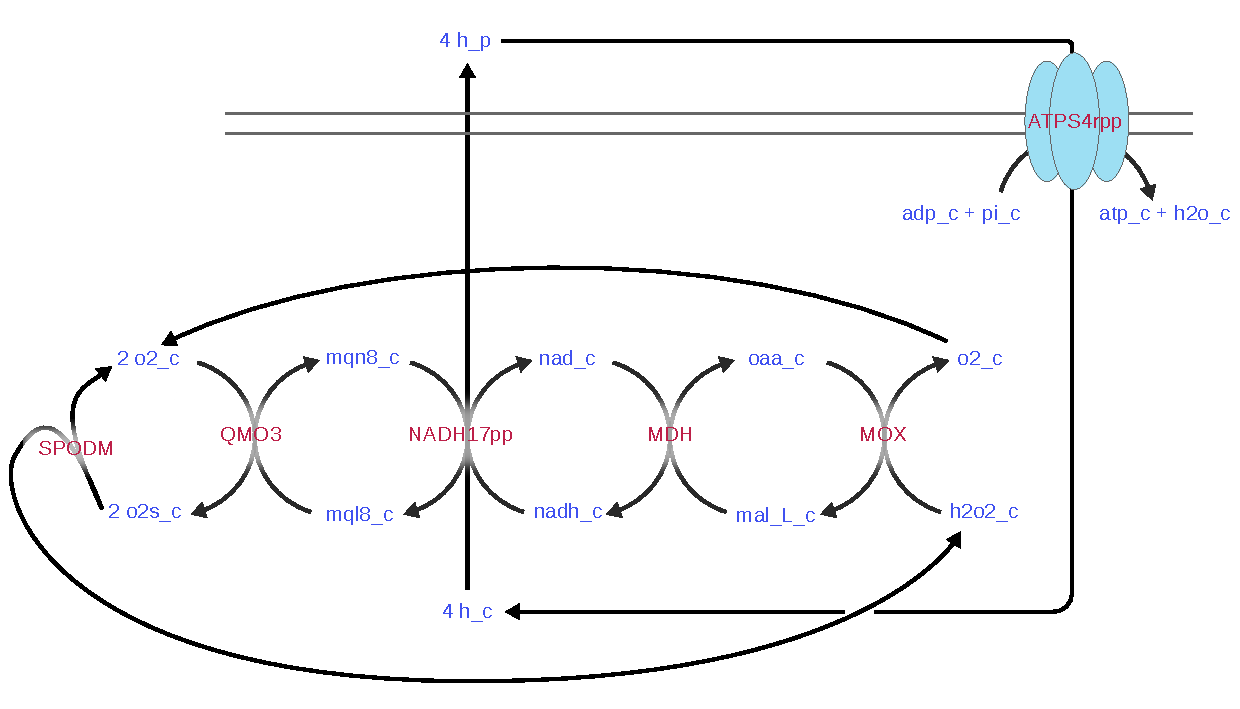
\includegraphics[width=6in]{figure2.pdf}
 	\caption{\csentence{An Energy Generating Cycle.}
 		If the reaction SPODM is not removed from the model iJO1366, it can
 		be used in this unrealistic pathway that generates ATP without any
 		external input.}
 	\label{fig:egc_example}
\end{figure*}

In this EGC, the Malate oxidase (MOX) reaction is used in the direction of oxaloacetate reduction. As was suggested previously \cite{Fritzemeier2017-ba}, constraining the reaction to be irreversible only in the direction of malate oxidation (after all, its $\Delta_r G'^\circ$ is approximately $-100$ kJ/mol) would solve this problem and eliminate the EGC from the solution space.

Nevertheless, many EGCs cannot be solved by constraining the direction of one thermodynamically irreversible reaction. Before giving an example for such a case, we must first explain the notion of \emph{distributed thermodynamic bottlenecks}.


\subsection*{Distributed Thermodynamic Bottlenecks}
What are distributed thermodynamic bottlenecks \cite{Mavrovouniotis1993-zq, Mavrovouniotis1996-dq}?
\elad{continue...}

\subsection*{Thermodynamic Flux Balance Analysis (TFBA)}

\elad{Talk about Energy Balance Analysis \cite{Beard2002-xt}. Talk about the duality paper \cite{Warren2007-wm}}
Thermodynamic FBA (also known as Thermodynamic-based Metabolic Flux Analysis \cite{Henry2007-xp}) was designed to deal with thermodynamically infeasible flux solutions. However, its widespread adoption has been hampered by the requirement for thermodynamic parameters. The set of equations that describe TFBA are:
\begin{eqnarray}
\textbf{TFBA:~~} && \nonumber\\
\mathbf{S} \cdot \mathbf{v} &=& \mathbf{0}  \label{eq:tfba1} \\
\mathbf{0} ~\leq~ \mathbf{v} &\leq & \mathbf{z} \cdot v_{max} \label{eq:tfba2} \\
\Sint^\top \cdot \mathbf{\Delta_f G'} &<& \kappa \cdot (1-\mathbf{z_{int}}) \label{eq:tfba3} \\
\mathbf{\Delta_f G'}& \geq & \mathbf{\Delta_f G'^\circ} + RT \cdot \ln(\mathbf{B_{low}}) \label{eq:tfba4} \\
\mathbf{\Delta_f G'}& \leq & \mathbf{\Delta_f G'^\circ} + RT \cdot \ln(\mathbf{B_{high}}) \label{eq:tfba5}
\end{eqnarray}
where the constants are the stoichiometric matrix of internal reactions $\Sint \in \mathcal{R}^{m \times r}$  and the vector of standard Gibbs energies of formation $\mathbf{\Delta_f G'^\circ}$ (in units of kJ/mol), the gas constant $R$ = 8.31 J/mol/K and temperature $T$ = 300 K. The variables are the flux vector $\mathbf{v} \in \mathcal{R}_{+}^{r}$, the vector of binary reaction indicators $\mathbf{z} \in \{0,1\}^{r}$, and the vector of Gibbs energies of formation $\mathbf{\Delta_f G'}$. Equation \ref{eq:tfba2} makes sure that $z_i$ would be 1 whenever there is a non-zero flux in reaction $i$. Equation \ref{eq:tfba3} represents the second law of thermodynamics. This is made clear by the fact that multiplying the stoichiometric matrix by the vector of chemical potentials gives the vector of changes in reaction Gibbs energies for all reactions in the model, i.e. $\mathbf{\Delta_r G'} \equiv \Sint^\top \cdot \mathbf{\Delta_f G'}$. Then, for every reaction whose flux is not zero (which forces $z_i = 1$), the constraint would be $\Delta_r G'_i < 0$ -- as dictated by the second law. $\kappa$ is a large scalar (orders of magnitude larger than all $\mathbf{\Delta_f G'^\circ}$ values), and is there to make sure the constraint is easily satisfied for inactive reactions (i.e. such that $\Delta_r G'_i < \kappa$ will always be true). Note that in the original paper \cite{Henry2007-xp} the letter used for this large scalar is $K$, and we chose to replace it with $\kappa$ in order to avoid any confusion with the temperature unit (Kalvin).  Finally, Equations \ref{eq:tfba4}-\ref{eq:tfba5} represent the bounds on the Gibbs energies of formation, assuming the concentration of each metabolite is between $B_{low,i}$ and $B_{high,i}$.

At first, it might seem strange that all fluxes are constrained to be non-negative (Equation \ref{eq:tfba2}), as many of the reactions in standard network reconstructions are reversible. This stems from the fact that non-negative fluxes are essential in order to formulate the thermodynamic constraints in a MILP framework. Fortunately, there is a simple procedure that converts reversible models to equivalent irreversible ones, simply by splitting every reversible reaction into two opposite irreversible ones, and treating the difference between their fluxes as the net flux. In the case of TFBA, the thermodynamic constraints will also make sure that only one of these opposite reactions is active ($v_i > 0$) at a time. For this reason, one must not equate these two opposite reactions to be the microscopic fluxes (i.e. the forward and backward rate that co-exist in reversible kinetic rate laws, and whose ratio is determined by the $\Delta_r G'$ \cite{Beard2007-kp}). 

While the stoichiometric matrix ($\mathbf{S}$) and general flux constraints are exactly the same as in the standard FBA formulation, $\mathbf{\Delta_f G'^\circ}$ comes as an additional requirement for running TFBA. Unfortunately, we still lack precise measurement for many of the compounds comprising biochemical networks, and computational methods that estimate $\mathbf{\Delta_f G'^\circ}$ \cite{Jankowski2008-hd,Noor2012-mp,Noor2013-an,Jinich2014-nv} are far from perfect and sometimes introduce significant errors. The fact that TFBA also adds one boolean variable for each reaction in the model definitely doesn't help either, since solving the LP becomes much harder, requires a good MILP solver, and takes much longer than standard FBA. Due to the effort involved, and the unclear benefit of the method, TFBA has not gained a wide audience of users so far.

\subsection*{Loopless Flux Balance Analysis (ll-FBA)}
In light of these caveats, it might be easier to understand why ll-FBA was introduced four years \emph{after} TFBA \cite{Schellenberger2011-bq}. Essentially, the loopless algorithm uses exactly the same MILP design as TFBA, while forgoing the actual thermodynamic values. This way, thermodynamically infeasible internal (Type III) cycles are eliminated, while all other pathways are kept \cite{Noor2012-qb}. The set of equations describing ll-FBA are:
\begin{eqnarray}
\textbf{ll-FBA:~~~~~~~~} && \nonumber\\
\mathbf{S} \cdot \mathbf{v} &=& \mathbf{0} \label{eq:llfba1} \\
\mathbf{0} ~\leq~ \mathbf{v} &\leq & \mathbf{z} \cdot v_{max} \label{eq:llfba2} \\
\Sint ^\top \cdot \mathbf{\Delta_f G'} &\leq & \kappa - (\kappa+1)\mathbf{z_{int}} \label{eq:llfba3}
\end{eqnarray}
where all variables and constants are the same as in equations \ref{eq:tfba1}-\ref{eq:tfba4}, and $\mathbf{\Delta_f G'} \in \mathcal{R}^{m}$. This formal representation of ll-FBA might seem different from Schellenberger et al. \cite{Schellenberger2011-bq}, but is actually equivalent. These changes facilitate the comparison to the TFBA algorithm. First, as in TFBA, we make the stoichiometric model irreversible, by duplicating each reversible reaction into two irreversible ones with opposite directionality. In addition, the original formulation contained a variable $\mathbf{G} \in \mathcal{R}^{r}$ which was constrained to be orthogonal to the null-space of $\Sint$. According to the fundamental theorem of linear algebra, the image of $A^\top$ is orthogonal to the null-space of $A$. Therefore, we chose to replace $\mathbf{G}$ with the expression $\Sint^\top \cdot \mathbf{\Delta_f G'}$, which is a general formula for a vector from the image of $\Sint^\top$.

\paragraph{A comparison ll-FBA to TFBA} After establishing the equivalence between Equations \ref{eq:llfba1}-\ref{eq:llfba3} and the original formulation of ll-FBA in \cite{Schellenberger2011-bq}, we can move on to compare them to TFBA (i.e. Equations \ref{eq:tfba1}-\ref{eq:tfba4}). One finds two main differences. First, the upper bound on $G_i$ in Equation \ref{eq:llfba3} is a bit tighter when $z_i = 1$ (i.e. -1 instead of 0). This constraint was added in \cite{Schellenberger2011-bq} to avoid the degenerate solution $G_i = 0$ for all $i$, and the margin (-1) was chosen arbitrarily since it does not affect the results. A more significant difference, is that in ll-FBA, there are no bounds on $\mathbf{\Delta_f G'}$ (i.e. as in Equations \ref{eq:tfba4}-\ref{eq:tfba5}). Therefore, ll-FBA is equivalent to TFBA with infinite concentration bounds (and consequently, the values of $\mathbf{\Delta_f G'^\circ}$ have no effect and can be set arbitrarily to 0).

\paragraph{Limited adoption of ll-FBA} Although ll-FBA requires no extra parameters compared to FBA, and its implementation is streamlined as part of the COBRA toolbox, it has yet to become mainstream. A plausible explanation would be that there is an alternative method for eliminating internal cycles in FBA solutions, which does not require an MILP, and can be easily implemented: after applying additions constraints that  define the relevant solution space (e.g. realizing the maximal biomass yield, or keeping all exchange fluxes constant), find a solution with the minimum sum of absolute (or squared) fluxes \cite{Holzhutter2004-qj}. Implementations of this principle with slight variations have been presented under different names such as parsimonious FBA \cite{Lewis2010-rx, Schuetz2012-sv} or CycleFreeFlux \cite{Desouki2015-lh}.

\section*{Results}

\subsection*{A compromise between ll-FBA and TFBA}
So, is there a version of thermodynamic-based FBA, that doesn't require a large set of extra (unknown) parameters, and still has a clear benefit over the standard tools that ignore thermodynamics? Here, we propose such a compromise, by relaxing the majority of second-law constraints (i.e. Equation \ref{eq:tfba3}) and keeping only a few important ones. We will show that this method, which we denote st-FBA (semi-thermodynamic Flux Balance Analysis), is sufficient to eliminate energy generating cycles, while requiring a relatively small set of heuristic assumptions and thermodynamic constants.

First, one must define a set of energy currency metabolites. Although the definition is somewhat heuristic, most biologists would agree that the following are energy equivalents: ATP, pyrophosphate, and a gradient of protons across the membrane. Other specific energy-carrying currency metabolites can be added to the list if desired. Next, we must bound the chemical potential ($\mathbf{\Delta_f G'}$) of these currency metabolites and all their associated degraded forms (see Table \ref{table:potentials}). Note that we chose the chemical potential at 1 mM concentration in an aqueous solution, which is a typical concentration for co-factors in \emph{E. coli} \cite{Bennett2009-rm}. Although it is possible to use the exact measured concentration of each of these metabolites, the effect on the st-FBA results would be at most very minor. 

Finally, we fix the values in the $\mathbf{G_f}$ vector only for these metabolites from the table, while the rest of the values remain free.
\begin{eqnarray}
\textbf{st-FBA:}~~\nonumber\\
\mathbf{S} \cdot \mathbf{v} &=& \mathbf{0} \label{eq:stfba1}\\
\mathbf{0} ~\leq~ \mathbf{v} &\leq & \mathbf{z} \cdot v_{max} \label{eq:stfba2}\\
\Sint^\top \cdot \mathbf{\Delta_f G'} &\leq & \kappa \cdot(1 - \mathbf{z_{int}}) \label{eq:stfba3}\\
\forall i~\textsf{in Table \ref{table:potentials}}\nonumber\\
\Delta_f G'_i & \geq & \Delta_f G'^\circ_i + RT \ln(B_{low,i}) \\
\Delta_f G'_i & \leq & \Delta_f G'^\circ_i + RT \ln(B_{high,i})
\end{eqnarray}
So st-FBA is very similar to TFBA, except that only the energy currency metabolites have predefined bounds on their formation energies. In fact, since the concentrations of these metabolites tend to be tightly controlled by homeostasis, it is recommended to set them to fixed concentrations (i.e. by setting the lower and upper bounds to the same value).

\subsection*{Implementation of st-FBA}
The semi-thermodynamic Flux Balance Analysis algorithm was implemented using COBRApy \cite{Ebrahim2013-vw}.

\subsection{Gibbs Energy of Formation Variation Analysis (GVA)}

\wolf{I think one thing would be nice to show or discuss: naively, one might think that constraining the chemical potentials of cofactors has only an effect on reactions that contain ONLY cofactors; that this determines the usage / flux directions in these reaction; and that this then has effects on other parts of the network. But in fact (that's at least how I understand your method) it looks like there are much more effects because every metabolite (even though its chemical potential can be freely chosen) must have one definite value of its chemical potential - such that the entire system becomes much more constrained.}
\elad{I think I can perform a kind of "FVA" on the potentials to see the ranges. It's also nice to compare that to the actual formation energies...}
%%%%%%%%%%%%%%%%%%%%%%%%%%%%%%%%%%%%%%%%%%%%%%
%%                                          %%
%% Backmatter begins here                   %%
%%                                          %%
%%%%%%%%%%%%%%%%%%%%%%%%%%%%%%%%%%%%%%%%%%%%%%

\begin{backmatter}

\section*{Competing interests}
  The authors declare that they have no competing interests.

\section*{Author's contributions}
EN performed the study and wrote this paper.

\section*{Acknowledgements}
I thank Wolfram Liebermeister, Arren Bar-Even, Dimitris Christodoulou, Mattia Zampieri for very helpful discussions and suggestions.

%%%%%%%%%%%%%%%%%%%%%%%%%%%%%%%%%%%%%%%%%%%%%%%%%%%%%%%%%%%%%
%%                  The Bibliography                       %%
%%                                                         %%
%%  Bmc_mathpys.bst  will be used to                       %%
%%  create a .BBL file for submission.                     %%
%%  After submission of the .TEX file,                     %%
%%  you will be prompted to submit your .BBL file.         %%
%%                                                         %%
%%                                                         %%
%%  Note that the displayed Bibliography will not          %%
%%  necessarily be rendered by Latex exactly as specified  %%
%%  in the online Instructions for Authors.                %%
%%                                                         %%
%%%%%%%%%%%%%%%%%%%%%%%%%%%%%%%%%%%%%%%%%%%%%%%%%%%%%%%%%%%%%

% if your bibliography is in bibtex format, use those commands:
\bibliographystyle{bmc-mathphys} % Style BST file (bmc-mathphys, vancouver, spbasic).
\bibliography{stfba_lib}      % Bibliography file (usually '*.bib' )
% for author-year bibliography (bmc-mathphys or spbasic)
% a) write to bib file (bmc-mathphys only)
% @settings{label, options="nameyear"}
% b) uncomment next line
%\nocite{label}

% or include bibliography directly:
% \begin{thebibliography}
% \bibitem{b1}
% \end{thebibliography}

%%%%%%%%%%%%%%%%%%%%%%%%%%%%%%%%%%%
%%                               %%
%% Figures                       %%
%%                               %%
%% NB: this is for captions and  %%
%% Titles. All graphics must be  %%
%% submitted separately and NOT  %%
%% included in the Tex document  %%
%%                               %%
%%%%%%%%%%%%%%%%%%%%%%%%%%%%%%%%%%%

%%
%% Do not use \listoffigures as most will included as separate files


%%%%%%%%%%%%%%%%%%%%%%%%%%%%%%%%%%%
%%                               %%
%% Tables                        %%
%%                               %%
%%%%%%%%%%%%%%%%%%%%%%%%%%%%%%%%%%%

%% Use of \listoftables is discouraged.
%%
\section*{Tables}

\begin{table}[h!]
\caption{Example of an Energy Generating Cycle that is possible in iJO1366}
\begin{tabular}{l|l}
\label{table:egc_example}
Reaction & Formula\\\hline
MDH & mal\_\_L-c + nad\_c = h\_c + nadh\_c + oaa\_c\\
MOX	& h2o2\_c + oaa\_c = mal\_\_L\_c + o2\_c\\
Htex	& h\_e = h\_p\\
EX\_h\_e & = h\_e\\
SPODM & 2.0 h\_c + 2.0 o2s\_c = h2o2\_c + o2\_c\\
NADH17pp & 4.0 h\_c + mqn8\_c + nadh\_c = mql8\_c + nad\_c + 3.0 h\_p\\
QMO3 & mql8\_c + 2.0 o2\_c = 2.0 h\_c + mqn8\_c + 2.0 o2s\_c\\
ATPS4rpp & adp\_c + pi\_c + 4.0 h\_p = atp\_c + 3.0 h\_c + h2o\_c\\\hline
Total & adp\_c + pi\_c = atp\_c + h2o\_c
\end{tabular}
\end{table}


\begin{table}[h!]
\caption{Table of currency metabolites, their standard Gibbs energies of formation, and bounded by their typical concentrations \cite{Bennett2009-rm}.}
\begin{tabular}{l|c|c|r}
\label{table:potentials}
\textbf{metabolite} & $\mathbf{B_{low}}$ & $\mathbf{B_{high}}$ & $\Delta_f G'^\circ$ [kJ/mol] \\ \hline
ATP & $9.63$ mM & $9.63$ mM & $-2296$ \\
ADP & $0.56$ mM & $0.56$ mM & $-1424$ \\
AMP & $0.28$ mM & $0.28$ mM & $-549$ \\
orthophosphate & $1$ mM & $10$ mM & $-1056$ \\
pyrophosphate & $1$ $\upmu$M & $1$ mM & $-1939$ \\
H$^+$ (cytoplasm) & $10^{-7.6}$ M $^\dagger$ & $10^{-7.6}$ M & $0$ \\
H$^+$ (extracellular) & $10^{-7.0}$ M & $10^{-7.0}$ M & $0$ \\
H$_2$O & 1 & 1 & $-157.6$
\end{tabular}
\begin{tablenotes}
\tiny
\item $\dagger$ Corresponding to pH 7.6, as measured by \citep{Wilks2007-lh}
\end{tablenotes}
\end{table}

%%%%%%%%%%%%%%%%%%%%%%%%%%%%%%%%%%%
%%                               %%
%% Additional Files              %%
%%                               %%
%%%%%%%%%%%%%%%%%%%%%%%%%%%%%%%%%%%

%%\section*{Additional Files}
%%  \subsection*{Additional file 1 --- Sample additional file title}
%%    Additional file descriptions text (including details of how to
%%    view the file, if it is in a non-standard format or the file extension).  This might
%%    refer to a multi-page table or a figure.
%%
%%  \subsection*{Additional file 2 --- Sample additional file title}
%%    Additional file descriptions text.


\end{backmatter}
\end{document}
